% Ordine di visita delle macro-celle nella strategia a serpentina (Sezione 1.7.3)
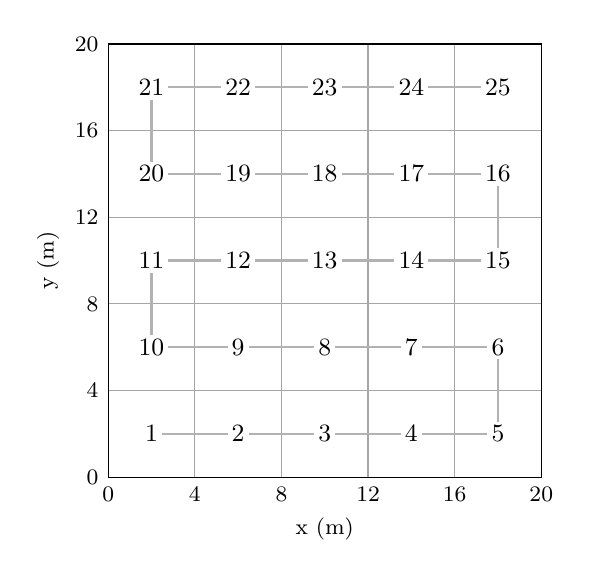
\begin{tikzpicture}[x=11mm, y=11mm, font=\small]
    % griglia 5 x 5 di macro-celle da 4 m
    \draw[step=1, gray!70] (0,0) grid (5,5);
    \draw (0,0) rectangle (5,5);

    % percorso a serpentina tra i centri delle macro-celle
    \draw[gray!60, line width=0.8pt]
        (0.5,0.5) -- (4.5,0.5) -- (4.5,1.5) -- (0.5,1.5) -- (0.5,2.5) -- (4.5,2.5)
        -- (4.5,3.5) -- (0.5,3.5) -- (0.5,4.5) -- (4.5,4.5);

    % numero d'ordine di ogni macro-cella
    \foreach \row in {0,...,4} {
        \foreach \col in {0,...,4} {
            \pgfmathtruncatemacro{\pos}{mod(\row,2) == 0 ? \col : 4 - \col}
            \pgfmathtruncatemacro{\num}{\row*5 + \pos + 1}
            \node[fill=white, inner sep=1.5pt] at (\col+0.5, \row+0.5) {\num};
        }
    }

    % coordinate in metri
    \foreach \i in {0,...,5} {
        \pgfmathtruncatemacro{\m}{4*\i}
        \node[below, font=\footnotesize] at (\i,0) {\m};
        \node[left, font=\footnotesize] at (0,\i) {\m};
    }
    \node[below=4mm, font=\footnotesize] at (2.5,0) {x (m)};
    \node[left=5mm, rotate=90, anchor=south, font=\footnotesize] at (0,2.5) {y (m)};
\end{tikzpicture}
